\documentclass[cic,tc]{iiufrgs}
\usepackage[utf8]{inputenc}   % pacote para acentuação
\usepackage{graphicx}         % pacote para importar figuras
\usepackage{times}            % pacote para usar fonte Adobe Times
\usepackage{algpseudocode}
% \usepackage{palatino}
% \usepackage{mathptmx}       % p/ usar fonte Adobe Times nas fórmulas
\usepackage[alf,abnt-emphasize=bf]{abntex2cite}	% pacote para usar citações abnt

%
% Informações gerais
%
\title{Estudo e otimização dos softwares de análise filogenética do Hospital de
Clínicas de Porto Alegre}

\author{Farah}{Alef}

% orientador e co-orientador são opcionais (não diga isso pra eles :))
\advisor[Prof.~Dr.]{Geyer}{Claudio Fernando Resin}
\coadvisor[Prof.~Dr.]{Anjos}{Julio Cesar Santos}

% a data deve ser a da defesa; se nao especificada, são gerados
% mes e ano correntes
\date{novembro}{2021}

% o local de realização do trabalho pode ser especificado (ex. para TCs)
% com o comando \location:
\location{Porto Alegre}{RS}

% itens individuais da nominata podem ser redefinidos com os comandos
%
% palavras-chave
% iniciar todas com letras minúsculas, exceto no caso de abreviaturas
%
\keyword{bioinformática}
\keyword{otimização}
\keyword{paralelismo}
%\keyword{}

%\settowidth{\seclen}{1.10~}

\begin{document}

% folha de rosto
% às vezes é necessário redefinir algum comando logo antes de produzir
% a folha de rosto:
% \renewcommand{\coordname}{Coordenadora do Curso}
\maketitle

% dedicatoria
% \clearpage
% \begin{flushright}
%     \mbox{}\vfill
%     {\sffamily\itshape
%       ``If I have seen farther than others,\\
%       it is because I stood on the shoulders of giants.''\\}
%     --- \textsc{Sir~Isaac Newton}
% \end{flushright}

% agradecimentos
%\chapter*{Agradecimentos}
%Agradeço ao \LaTeX\ por não ter vírus de macro\ldots

% resumo na língua do documento
\begin{abstract}
  A análise filogenética compreende o estudo da evolução dos organismos e suas
  características. Neste trabalho foi realizado um estudo e otimização dos
  problemas de desempenho presentes nos softwares de análise filogenética
  utilizados pelo grupo de pesquisa em genética do Hospital de Clínicas de
  Porto Alegre (HCPA), empregando para isso técnicas de processamento paralelo.
  O tempo total da análise realizada pelo grupo foi reduzido de X para Y. % TODO
\end{abstract}

% resumo na outra língua
% como parametros devem ser passados o titulo e as palavras-chave
% na outra língua, separadas por vírgulas
\begin{englishabstract}{Study and optimization of the phylogenetic analysis software used by Hospital de Clínicas de Porto Alegre}{Bioinformatics, optimization, parallelism} Phylogenetic analysis comprises the study of the evolution of living beings and their characteristics. In this paper we studied and optimized the performance bottlenecks present in the phylogenetic analysis software used by the genetics research group from the Hospital de Clínicas de Porto Alegre, using parallel programming techniques. The analysis total execution time was reduced from X to Y. % TODO
\end{englishabstract}

% lista de figuras
\listoffigures

% lista de tabelas
\listoftables

% lista de abreviaturas e siglas
% o parametro deve ser a abreviatura mais longa
\begin{listofabbrv}{HPCA}
    \item[HCPA] Hospital de Clínicas de Porto Alegre
    \item[PAML] \textit{Phylogenetic Analysis By Maximum Likelihood}
    \item[CPU] \textit{Central Processing Unit}
    \item[GPU] \textit{Graphics Processing Unit}
    \item[BFGS] Broyden–Fletcher–Goldfarb–Shanno
    \item[DNA] Ácido desoxirribonucleico
    \item[RNA] Ácido ribonucleico
\end{listofabbrv}

% idem para a lista de símbolos
\begin{listofsymbols}{$\omega$}
    \item[$\omega$] Taxa de substituição
    \item[$dN$] Substituições não-sinônimas
    \item[$dS$] Substituições sinônimas
\end{listofsymbols}

% sumario
\tableofcontents

% aqui comeca o texto propriamente dito

% introducao
\chapter{Introdução}

Neste trabalho foi realizado um estudo e otimização dos problemas de desempenho
presentes nos softwares de análise filogenética utilizados pelo grupo de
pesquisa em genética do Hospital de Clínicas de Porto Alegre (HCPA), empregando
para isso técnicas de processamento paralelo e distribuído sempre que viável.

A análise realizada pelo grupo emprega softwares diversos, que apresentavam
tempos de execução proibitivamente lentos - a análise de um único gene levava
até dois dias, enquanto o grupo pretende analisar centenas de genes - além de
uso de memória proibitivamente elevado em certas etapas da análise. Neste
trabalho foram estudados os softwares utilizados pelo grupo, realizando para
tal revisão bibliográfica sobre o tema e análises de desempenho aprofundadas.
Além disso, foi estudada a possibilidade de paralelização dos algoritmos
empregados visando a redução do seu tempo de execução, e, sempre que possível,
foi implementada tal paralelização, seguida de novas análises, tanto da
corretude da nova implementação como das melhorias de desempenho obtidas.

Por fim, as otimizações resultantes deste trabalho nos diversos softwares que
compõem a análise filogenética foram reunidas em uma ferramenta para execução
de ponta a ponta da análise. Com isso, obteve-se uma redução significativa do
tempo total de execução da análise, que de vários dias passou a levar algumas
horas.

\section{Análise filogenética}

A análise filogenética, cujos softwares associados foram objeto de estudo desse
trabalho, compreende o estudo da evolução de um ou mais organismos e suas
características. Os pesquisadores do HCPA realizam tal estudo evolutivo a nível
molecular, através da comparação da informação genética de diferentes linhagens
ou populações de um ser.

A informação genética presente no DNA dos seres vivos, objeto de estudo do
grupo de pesquisa do HCPA, é utilizada no processo de síntese proteica, onde os
códons (tripla de nucleotídeos) presentes no RNA mensageiro, gerado a partir do
DNA, determinam a síntese de aminoácidos específicos, componentes das
proteínas, macromoléculas fundamentais à vida.

Existem quatro tipos de nucleotídeos no código genético, formados por adenina
(A), guanina (G), uracila (U), e citosina (C). Dessa forma, existem $4^3 = 64$
códons distintos, dos quais três sâo códons de terminação, que indicam o fim da
etapa de tradução na síntese protéica, enquanto os outros 61 códons traduzem
para um aminoácido específico.

Apenas 20 aminoácidos compõem as proteínas em seres vivos. Sendo assim, a
maioria dos aminoácidos é traduzido por mais de um códon. Em outras palavras, a
substituição de certos códons no DNA não produz alteração nos aminoácidos
gerados na síntese proteica.

As substituições que não geram alterações na síntese proteica são chamadas de
sinônimas ou silenciosas, enquanto as que modificam os aminoácidos gerados são
não-sinônimas. Acredita-se que as substituições sinônimas sejam mais comuns e
não sofram tanta pressão seletiva. A taxa de substituiçõs sinônimas e não
sinônimas $\omega = \frac{dN}{dS}$ é uma medida de seleção natual, conforme a
tabela abaixo.\cite{yang2002codon}

\begin{table}[h]
    \caption{Taxas de substituição}
    % OBS: não use \begin{center}, pois este aumenta o espaçamento entre a caption/legend e a tabela
    % Para figuras, a aparência é melhor com o espaçamento extra
    \centering
        \begin{tabular}{c|c}
          \hline
          \textit{Taxa}  &   \textit{Seleção} \\
          \hline
          \hline
          $\omega = 1$ & Seleção neutra \\
          $\omega < 1$ & Seleção negativa ou purificadora \\
          $\omega > 1$ & Seleção positiva \\
          \hline
        \end{tabular}
      \legend{Fonte: \cite{yang2002codon}}
    \label{tbl:ex1}
\end{table}

Existem diversos modelos de análise dessas substituições em diferentes
linhagens de um indivíduo, e variados softwares que os implementam. Esse
trabalho foca nos modelos e softwares de análise filogenética
utilizados pelo grupo do HCPA.

\section{Software utilizado e abordagens selecionadas}

\section{Pacote PAML}

O \textit{Phylogenetic Analysis by Maximum Likelihood} (PAML) é um pacote de
software com ferrametas para análise filogenética utilizando métodos
estatísticos de máxima verossimilhança.\cite{yang2007paml} Dentre
outras ferramentas disponíveis no pacote se destaca o codeml,
amplamente utilizado na literatura.\cite{maldonado2016lmap}

Apesar de estatisticamente robusto,\cite{maldonado2016lmap} o codeml
possui implementação ingênua de métodos numéricos computacionalmente
custosos.\cite{yang2020paml} Para o caso de uso do grupo de pesquisa em
genética do HCPA, o tempo de execução é de vários dias.

Na literatura encontra-se implementações diversas que buscam melhorar o
desempenho do codeml. Em \cite{moretti2012gcodeml} os autores fornecem
uma solução para cluster; em \cite{maldonado2016lmap} é implementado uma
ferramenta para execução paralela de múltiplos \textit{jobs} do codeml
em uma única máquina (em CPU); em \cite{schabauer2012slimcodeml} os autores
re-escrevem o software melhorando sua organização e otimizando-o,
substituindo implementações ingênuas por aquelas de bibliotecas de métodos
numéricos como BLAS e LAPACK, e em \cite{valle2014optimization} os
mesmos autores fornecem uma implementação paralela (em CPU) para um
sub-conjunto de métodos do seu software.

Nesse trabalho foram exploradas todas as soluções supracitadas com exceção da
abordagem para cluster, visto que os pesquisadores do HCPA vem
utilizando um \textit{setup} com apenas uma máquina, além da solução em
questão ser customizada para um cluster específico ao qual os autores
desse trabalho não possuem acesso.

Além disso, nesse trabalho o codeml foi perfilado utilizando as ferramentas
callgrind e kcachegrind,\cite{weidendorfer2008sequential} para os dados
de entrada do caso de uso do grupo de pesquisa do HCPA. Com base no
resultado desse perfil de execução, foram implementadas e testadas
algumas abordagens de paralelismo em CPU das rotinas que consumiam o
maior tempo de execução do codeml, mas tal abordagem foi posteriormente
descartada em favor das soluções encontradas na literatura, conforme
descrito em \ref{subsec:codemlpar}. Uma abordagem para GPU foi estudada, mas igualmente
descartada em favor das soluções existentes, conforme descrito em \ref{subsec:codemlpar}.

\subsection{Perfil de execução e estudo de implementação paralela}
\label{subsec:codemlpar}

A fim de determinar os gargalos de desempenho do codeml para o caso de uso do
grupo de pesquisa do HCPA, foi traçado um perfil de execução da aplicação com
os dados de entrada fornecidos pelos pesquisadores do HCPA utilizando as
ferramentas callgrind e kcachegrind.\cite{weidendorfer2008sequential}

O perfil de execução revelou que $97,28\%$ do tempo de execução da aplicação
era dispendido na rotina \textit{ming2}. Um estudo do código fonte revela
que ela implementa o algoritmo de Broyden–Fletcher–Goldfarb–Shanno (BFGS), um
método numérico para resolução de problemas de otimização. Tal método possui,
no caso do codeml, duas sub-rotinas responsáveis por quase a totalidade de seu
tempo de execução: \textit{gradientB} e \textit{LineSearch2}.

A rotina \textit{gradientB}, responsável por $42,99\%$ do tempo total da
aplicação, implementa o cálculo do gradiente via diferenças finitas, enquanto
\textit{LineSearch2}, responsável por $53,27\%$ do tempo de execução,
implementa um método numérico de busca linear utilizando interpolação
quadrática, descrito em \cite{wolfe1978numerical}. A
figura~\ref{fig:kcachegrind} fornece uma visualização da pilha de chamadas em
questão.

\begin{figure}
  \caption{Pilha de chamadas do codeml}
    \begin{center}
        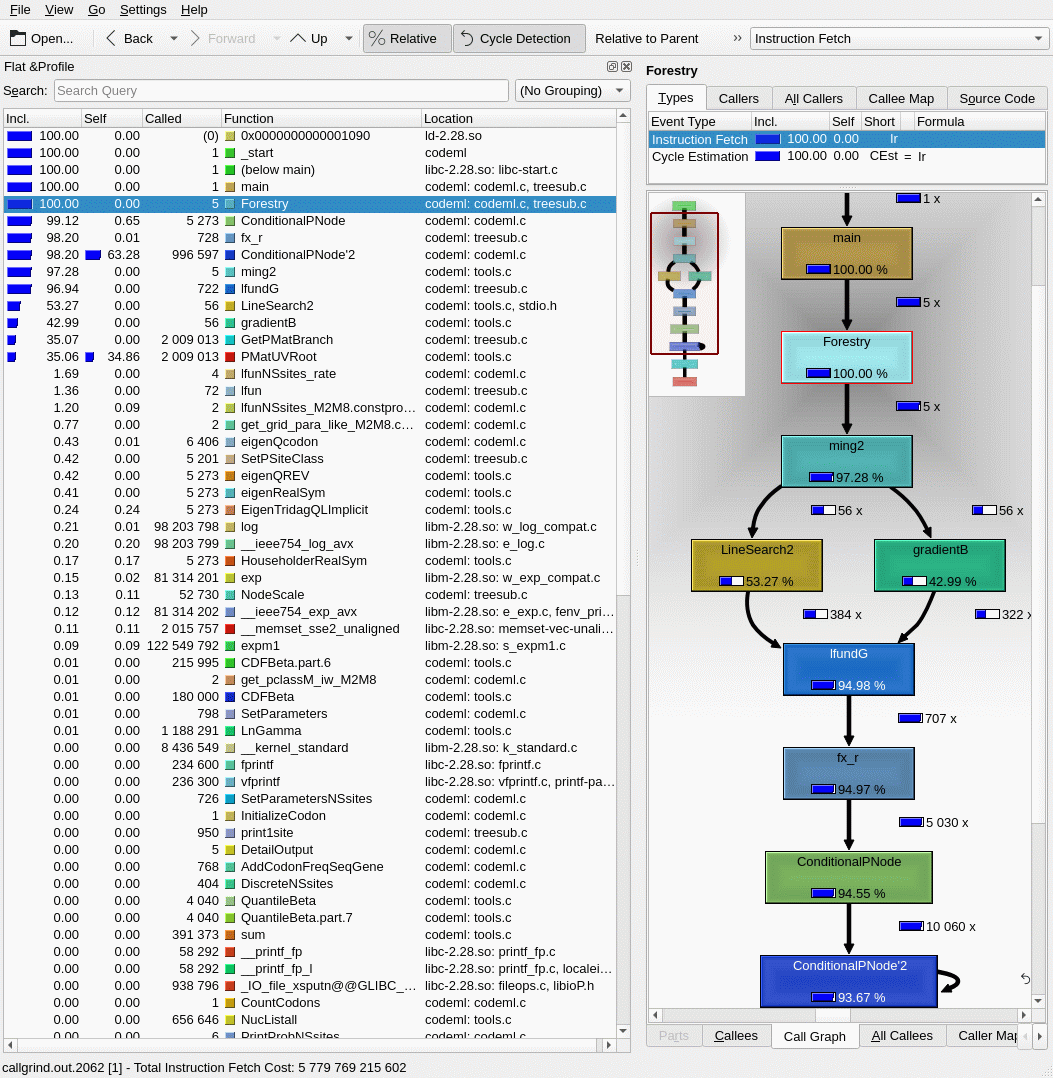
\includegraphics[width=0.3\linewidth]{img/kcachegrind.png}
    \end{center}
    \legend{Fonte: Os Autores}
    \label{fig:kcachegrind}
\end{figure}

Foi considerada uma implementação paralela para todos os métodos numéricos
supracitados. Em um primeiro momento o cálculo do gradiente foi paralelizado
utilizando OpenMP, um modelo de programação paralela para sistemas com
múltiplos processadores com memória compartilhada.\cite{chandra2001parallel} A
escolha se justifica pela implementação ser trivial.

A fim de garantir a corretude da implementação paralela, foram desenvolvidos
testes unitários para a função, utilizando dados de entrada arbitrários e
comparando os resultados da implementação sequencial e paralela. Os testes
revelaram que a implementação paralela gerava resultados diferentes da
sequencial. Um estudo da implementação revelou que ela está correta, mas a
função cujo grandiente está sendo calculado é implementada de forma não
\textit{thread-safe}, gerando condições de corrida.

Foi considerado a re-implementação das funções sendo diferenciadas, todavia, o
uso extensivo de variáveis globais e memória compartilhada na implementação
original do codeml demonstrou-se um grande obstáculo para essa abordagem, que
por isso foi abandonada.

A partir daí foram voltadas as atenções para \textit{LineSearch2}, mas não foi
encontrado na literatura implementações paralelas para o método descrito em
\cite{wolfe1978numerical}, e o algoritmo não é de paralelização trivial,
portando tal abordagem também foi abandonada.

Por fim, as atenções foram voltadas para o próprio \textit{ming2}, cujo método
numérico (BFGS) é iterativo. Foi realizada uma revisão bibliográfica, que
revelou implementações paralelas desse algoritmo para GPU em
\cite{fei2014parallel}. Todavia, além de complexa e de difícil adaptação para o
caso do codeml, o algoritmo não performa bem para entradas
pequenas,\cite{fei2014parallel}. que é o caso do codeml que trabalha com um
tamanho fixo de 61 (o número códons que traduzem para aminoácidos). Dessa
forma, essa abordagem também foi descartada.

Esgotadas todas possibilidades de paralelização das rotinas responsáveis por
quase a totalidade do tempo de execução do codeml para o caso de uso dos
pesquisadores do HCPA, partiu-se para um estudo das soluções presentes na
literatura.

\subsection{Estudo do desempenho de soluções da literatura}

A primeira aplicação a ser testada foi o
slimcodeml,\cite{schabauer2012slimcodeml} visto que o
fastcodeml\cite{valle2014optimization} não implementa os modelos necessários à
análise do grupo do HCPA. Utilizando os dados de entrada fornecidos por
pesquisadores do grupo, obteve-se uma redução no tempo total de execução de
16h38m para 5h24m, uma redução de 67,53\% no tempo de execução. Os testes foram
realizados em um ambiente controlado, de uso exclusivo dos autores, em uma
máquina TODO.

Em um segundo momento foi testado a aplicação TODO,\cite{maldonado2016lmap}

\section{Pacote samtools}

Outra aplicação utilizada no pipeline de análise do grupo de pesquisa em
genética é o pacote samtools,\cite{li2009sequence} aplicação amplamente
utilizada na literatura para análise de sequências
genéticas.\cite{danecek2021twelve} O samtoools e a ferramenta bcftools que o
acompanha são construídos em cima da biblioteca htslib, dos mesmos autores, que
permite a leitura e manipulação de arquivos de arquivos em formatos diversos
representando sequências genéticas alinhadas.\cite{danecek2021twelve}

Em mais detalhes, o formato SAM traz uma representação em texto-plano das
sequências genéticas alinhadas, o BAM é seu equivalente binário, e o CRAM é uma
versão binária com compressão. Enquanto o samtools manipula esses arquivos, o
bcftools manipula os arquivos no formato VCF, que armazena informação de
variantes genéticas em texto-plano, e no formato BCF, seu equivalente
binário.\cite{danecek2021twelve}

Os dados de sequenciamento genético utilizados como entrada no pipeline de
análise do grupo de pesquisa do HCPA são obtidos no formato CRAM do projeto
1000 Genomes, um esforço colaborativo internacional que visa sequenciar o
genoma humano e disponibilizar a informação publicamente.\cite{via20101000}

Nesse trabalho foi estutdado, otimizado, e paralelizado o pipeline de análise
do grupo de pesquisa do HCPA utilizando o samtools e o bcftools, reduzindo o
tempo de execução de vários dias para poucas horas.

\subsection{Fluxo de análise original}

O fluxo de análise original fornecido pelos pesquisadores pode ser dividido
em duas etapas. Na primeira etapa é executada uma conversão de formato de CRAM
para BAM utilizando o comando \textit{samtools view -b}, seguida de uma rotina
de indexação dos arquivos utilizando \textit{samtools index}.

Uma vez convertidos e indexados, cada arquivo de entrada é separado em 22
arquivos de saída, um para cada par de cromossomos autossômicos humanos,
utilizando o comando \textit{samtools view chr}. Essa etapa na sua forma
originalmente usada pelo grupo de pesquisa encontra-se reproduzida na
figura~\ref{fig:stage1_orig}.

\begin{figure}
  \caption{Fluxo de análise original, etapa 1}
    \begin{center}
      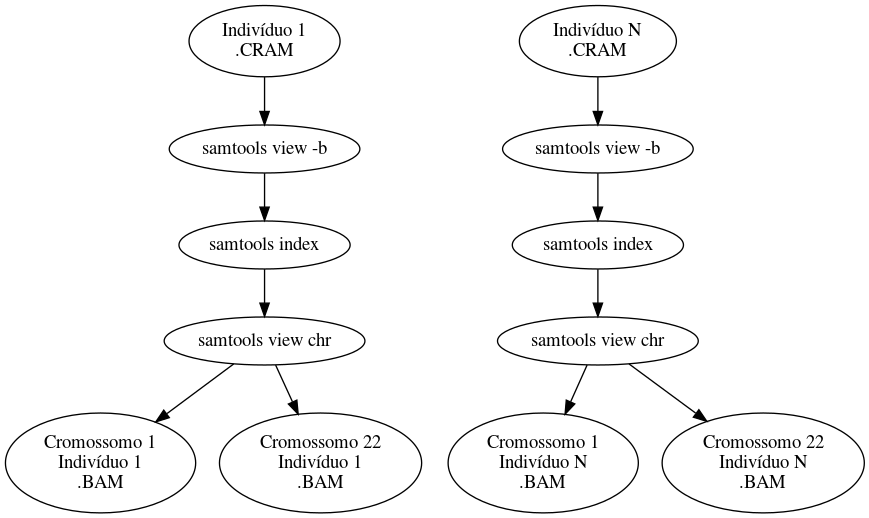
\includegraphics[width=0.85\linewidth]{img/stage1_orig.png}
    \end{center}
    \legend{Fonte: Os Autores}
    \label{fig:stage1_orig}
\end{figure}

Numa segunda etapa, para cada cromossomo são aglutinados os respectivos
arquivos de todos indivíduos, utilizando o comando \textit{samtools merge}.
Posteriormente esses arquivos são indexados, e os comandos \textit{bcftools
mpileup} e \textit{bcftools call} são invocados para executar a chamada de
variantes.

Por fim, o comando \textit{bcftools view} é executado para converter a saída do
formato BCF para VCF. Independente do número de arquivos de entrada, a saída é
sempre 22 arquivos. Essa etapa encontra-se reproduzida na
figura~\ref{fig:stage2_orig}.

\begin{figure}
  \caption{Fluxo de análise original, etapa 2}
    \begin{center}
      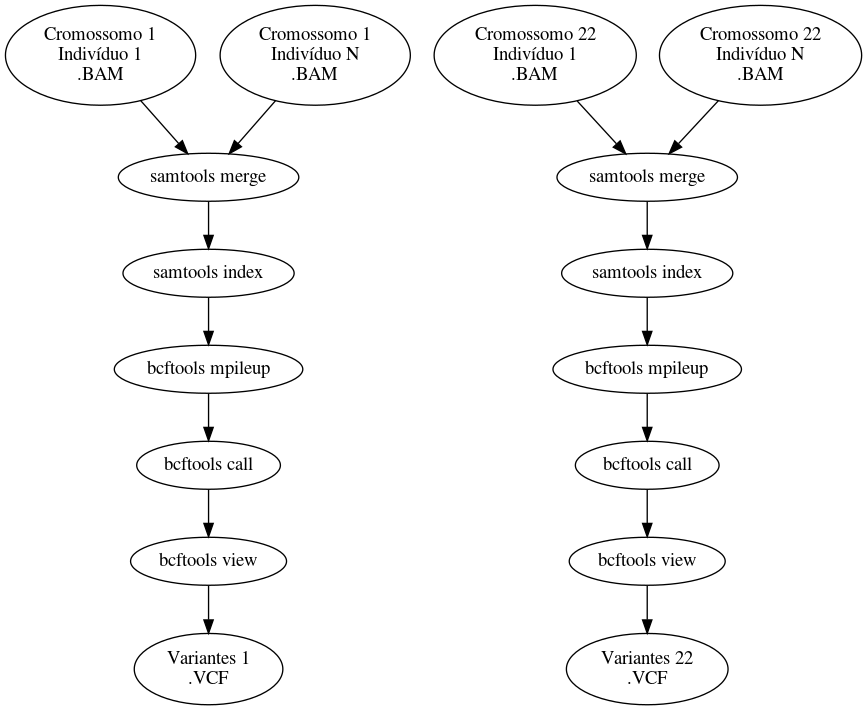
\includegraphics[width=0.85\linewidth]{img/stage2_orig.png}
    \end{center}
    \legend{Fonte: Os Autores}
    \label{fig:stage2_orig}
\end{figure}

\subsection{Fluxo de análise otimizado}

Através de um estudo da literatura e do manual das ferramentas utilizadas
percebeu-se oportunidade de melhorias no fluxo de análise utilizado pelos
pesquisadores. Em particular, em,\cite{danecek2021twelve} os autores observam
que o uso do comando \textit{samtools view -b}, para conversão de BAM para
CRAM, apesar de frequentemente presente em guias na internet é normalmente
desnecessário, uma vez que as ferramentas possuem suporte a CRAM.

Foram realizados testes de desempenho de cada uma das etapas do fluxo original
de análise, e a conversão de CRAM para BAM era particularmente custosa.
Observado isso, foi testado e comprovado que todo restante da análise poderia
ser executado sem essa etapa, observando o suporte para CRAM e comparando as
saídas do fluxo otimizado com o fluxo original.

Além disso, foi observado que ambas etapas eram embaraçosamente paralelas,
consistindo de passos independentes para cada arquivo de entrada. Como os
pesquisadores do HCPA possuem acesso a máquinas multiprocessadas, foi realizada
uma paralelização de ambas etapas utilizado GNU Parallel\cite{tange2011gnu}.  A
escolha dessa ferramenta se deu pela facilidade de uso, disponibilidade nos
ambientes usados pelos pesquisadores, e suporte a ajuste automático do número
de \textit{jobs} paralelos ao número de núcleos de processamento disponíveis.

Foi desenvolvida uma ferramenta para execução do fluxo de análise otimizado e
paralelizado. Um pseudo-código da ferramenta encontra-se reproduzido abaixo.

\begin{algorithmic}
  \For{CRAM EM
\end{algorithmic}


%% o `[h]' abaixo é um parâmetro opcional que sugere que o LaTeX coloque a
%% figura exatamente neste ponto do texto. Somente preocupe-se com esse tipo
%% de formatação quando o texto estiver completamente pronto (uma frase a mais
%% pode fazer o LaTeX mudar completamente de idéia sobre onde colocar as
%% figuras e tabelas)
%% \begin{figure}[h]
%\begin{figure}
%    \caption{Exemplo de figura desenhada com o environment \texttt{picture}.}
%    \begin{center}
%        \setlength{\unitlength}{.1em}
%        \begin{picture}(100,100)
%            \put(20,20){\circle{20}}
%            \put(20,20){\small\makebox(0,0){a}}
%            \put(80,80){\circle{20}}
%            \put(80,80){\small\makebox(0,0){b}}
%            \put(28,28){\vector(1,1){44}}
%        \end{picture}
%    \end{center}
%    \legend{Fonte: Os Autores}
%    \label{fig:ex2}
%\end{figure}
%
%Tabelas são construídas com praticamente os mesmos comandos. Ver a tabela \ref{tbl:ex1}.
%
%\begin{table}[h]
%    \caption{Uma tabela de Exemplo}
%    % OBS: não use \begin{center}, pois este aumenta o espaçamento entre a caption/legend e a tabela
%    % Para figuras, a aparência é melhor com o espaçamento extra
%    \centering
%        \begin{tabular}{c|c|p{5cm}}
%          \hline
%          \textit{Col 1}  &   \textit{Col 2}  &   \textit{Col 3} \\
%          \hline
%          \hline
%          Val 1           &   Val 2           & Esta coluna funciona como um parágrafo, tendo uma margem definida em 5cm. Quebras de linha funcionam como em qualquer parágrafo do tex. \\
%          Valor Longo     & Val 2             & Val 3 \\
%          \hline
%        \end{tabular}
%    \legend{Fonte: Os Autores}
%    \label{tbl:ex1}
%\end{table}
%

\bibliographystyle{abntex2-alf}
\bibliography{biblio}

\end{document}
